\documentclass[11pt]{article}
\usepackage[margin=1in]{geometry}
\usepackage{amsmath}
\usepackage[hidelinks]{hyperref}
\usepackage{xurl}
\usepackage{enumitem}
\usepackage{graphicx}
\usepackage{booktabs}
\usepackage{caption}
\usepackage{parskip}
\setlength{\parskip}{0.55em}

\title{\large AI-Orchestrated Diagnosis and Repair of a VQE Ansatz Failure Mode}
\author{}
\date{}

\begin{document}
\maketitle
\vspace{-2.2em}

\begin{abstract}
\noindent This is not a description of how AI agents \emph{could} be used for quantum research; it is an account of a specific project where one was, with the exact commands, failures, self-corrections, and validated results it produced. The underlying scientific result (Section~4) and the AI-orchestration process that produced it (Section~3) are both real and independently verifiable from the linked repository's commit history, run logs, and figures.
\end{abstract}

\section{The research question}
We study a chemistry-structured VQE ansatz (paired UCC doubles, PUCCD) across the potential energy surfaces of five molecules, H$_2$, LiH, BeH$_2$, HF, and BH (4--12 qubits, STO-3G basis), asking two questions: where does this ansatz fail, and is a given failure a fundamental limitation of what the ansatz can represent, or just an under-optimized run? The second question is rarely asked rigorously in small-scale VQE studies, and answering it is where AI-agent orchestration did the most work.

\section{Why this fits Track 1}
Everything in this project to date, including the ansatz fix in Section~4, has been validated only in noiseless classical simulation; no run has yet been submitted to real quantum hardware. The proposed extension (Section~5) is designed around a single-batched-job execution strategy chosen specifically to stay within free-tier QPU-time limits (all classical optimization performed in simulation; hardware used only for final verification), a direct, concrete push toward results that are harder to reach with today's NISQ devices under realistic access constraints.

\section{The AI-orchestration workflow (the ``how'')}
Three concrete episodes from this project illustrate what ``AI-orchestrated'' meant in practice: not passively running pre-written scripts, but actively managing long, failure-prone compute jobs and catching problems a human running the same pipeline could easily have missed.

\subsection{Long-running background job orchestration}
The full study spans 87 bond-length geometries across 5 molecules, each requiring a multi-restart classical optimization (up to 12 restarts $\times$ 250 iterations per geometry). Individual runs took minutes to hours depending on system load, with highly variable per-point timing (observed range: $\sim$150 seconds to over 2 hours for a single geometry under heavy system contention). The agent launched these as background processes, monitored them asynchronously without blocking on results, diagnosed and fixed real runtime bugs as they appeared (e.g.\ a silent NaN-target crash from 4 incomplete database records, a matplotlib API incompatibility), and re-launched corrected runs, all without requiring a human to babysit each step.

\subsection{Catching its own overstated statistical claim}
An early analysis reported a strong correlation between energy error and dipole-moment error (naive $p = 3.4\times10^{-5}$). Before accepting this, the agent identified that the underlying data points are \emph{not} independent samples, they lie along one smooth curve, and applied an autocorrelation-corrected effective-sample-size test (Pyper \& Peterman, 1998), which revised the result to a far less dramatic $p \approx 0.035$. A second self-audit, using outlier-robust Spearman rank correlation, further revealed that for two of the five molecules, an apparently strong raw correlation ($r = 0.75$--$0.91$) was being driven entirely by 1--2 extreme data points, not a real trend, and reported this honestly rather than keeping the more impressive-looking number.

\subsection{Refusing to accept a good-looking result at face value}
After a proposed ansatz fix showed a dramatic improvement (up to $446\times$ error reduction) at 4 hand-picked, previously catastrophic geometries, the agent did not stop there. It proactively re-ran the fix across the \emph{full} set of 55 geometries for the affected molecules, precisely because a 4-point spot check could have been cherry-picked or masked a regression elsewhere on the curve. The full-curve run (Section~4) confirmed the fix generalized, and also surfaced an honest partial result (one molecule improved substantially but not completely) that a less rigorous process might have glossed over.

\section{The scientific result this process produced (the ``what'')}
The orchestration process above was in service of a real finding, not just activity for its own sake. Two distinct ansatz failure modes were identified and mechanistically explained, then one was resolved.

\subsection{Two failure modes, explained by a classical (non-VQE) diagnostic}
LiH's energy and dipole error degrade \emph{gradually} as the bond stretches. HF and BH instead track the exact answer closely, then collapse sharply at one specific bond length. A purely classical diagnostic, the weight of the Hartree-Fock determinant in the exact (FCI) wavefunction, requiring no VQE run at all, explains why: HF and BH each undergo a genuine electronic-structure curve crossing at essentially the bond length where PUCCD fails; LiH does not.

\begin{figure}[h]
\centering
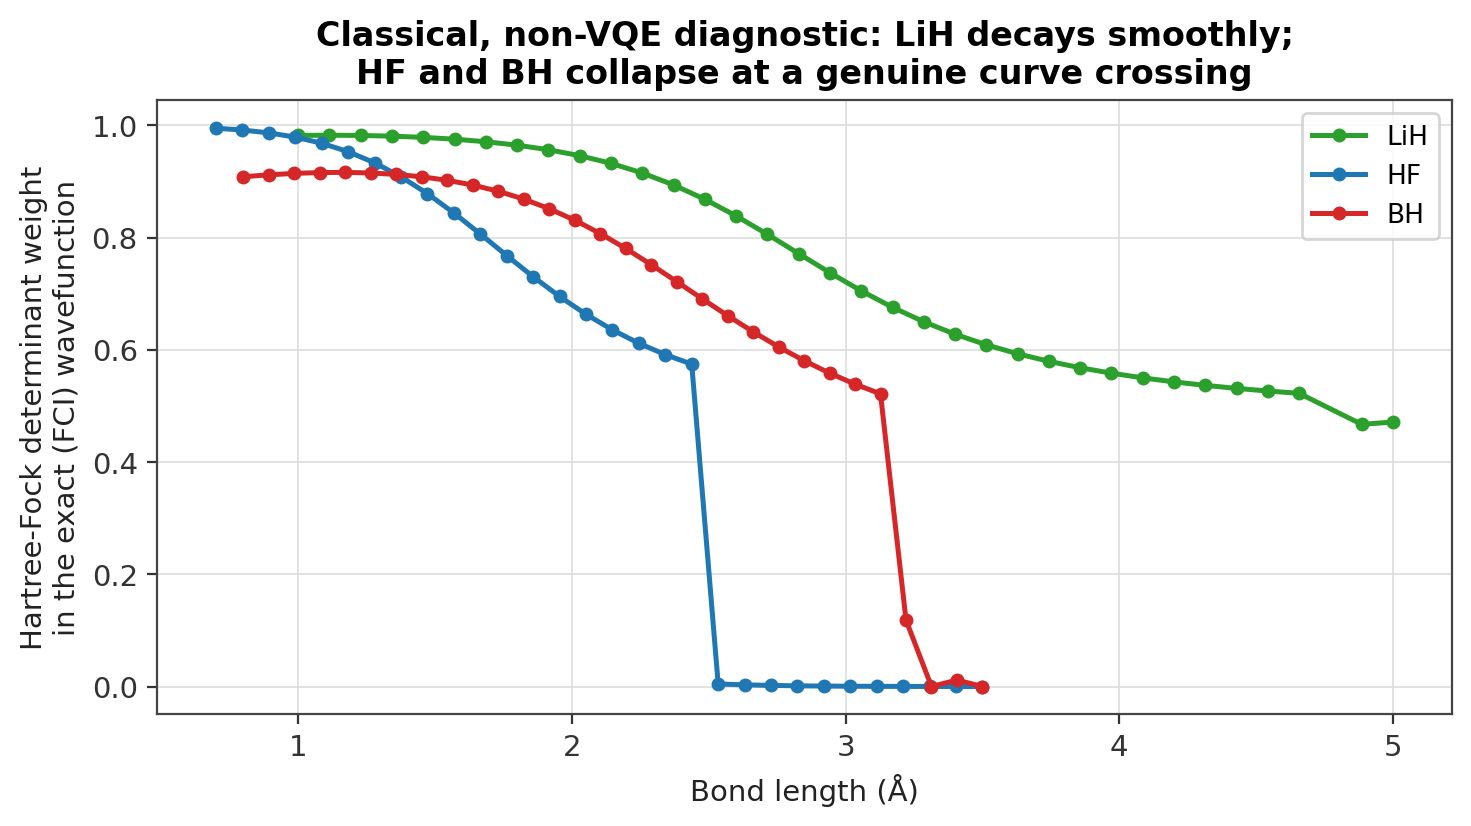
\includegraphics[width=0.62\textwidth]{results_decoupling/figures_proposal/multireference_mechanism.png}
\caption{Classical, non-VQE diagnostic: LiH decays smoothly; HF and BH collapse at a genuine curve crossing.}
\end{figure}

\subsection{A validated architectural fix}
PUCCD is restricted to paired double excitations and has no orbital-rotation degree of freedom, exactly the capability needed to track a wavefunction across a crossing. This is grounded directly in Anselmetti et al.\ (\textit{New J. Phys.} \textbf{23}, 113010, 2021), who show that pair-exchange-only and orbital-rotation-only ansätze are each individually non-universal, while their combination is. Adding single (orbital-rotation) excitations to PUCCD was tested across all affected geometries, not just the original failure points:

\begin{figure}[h]
\centering
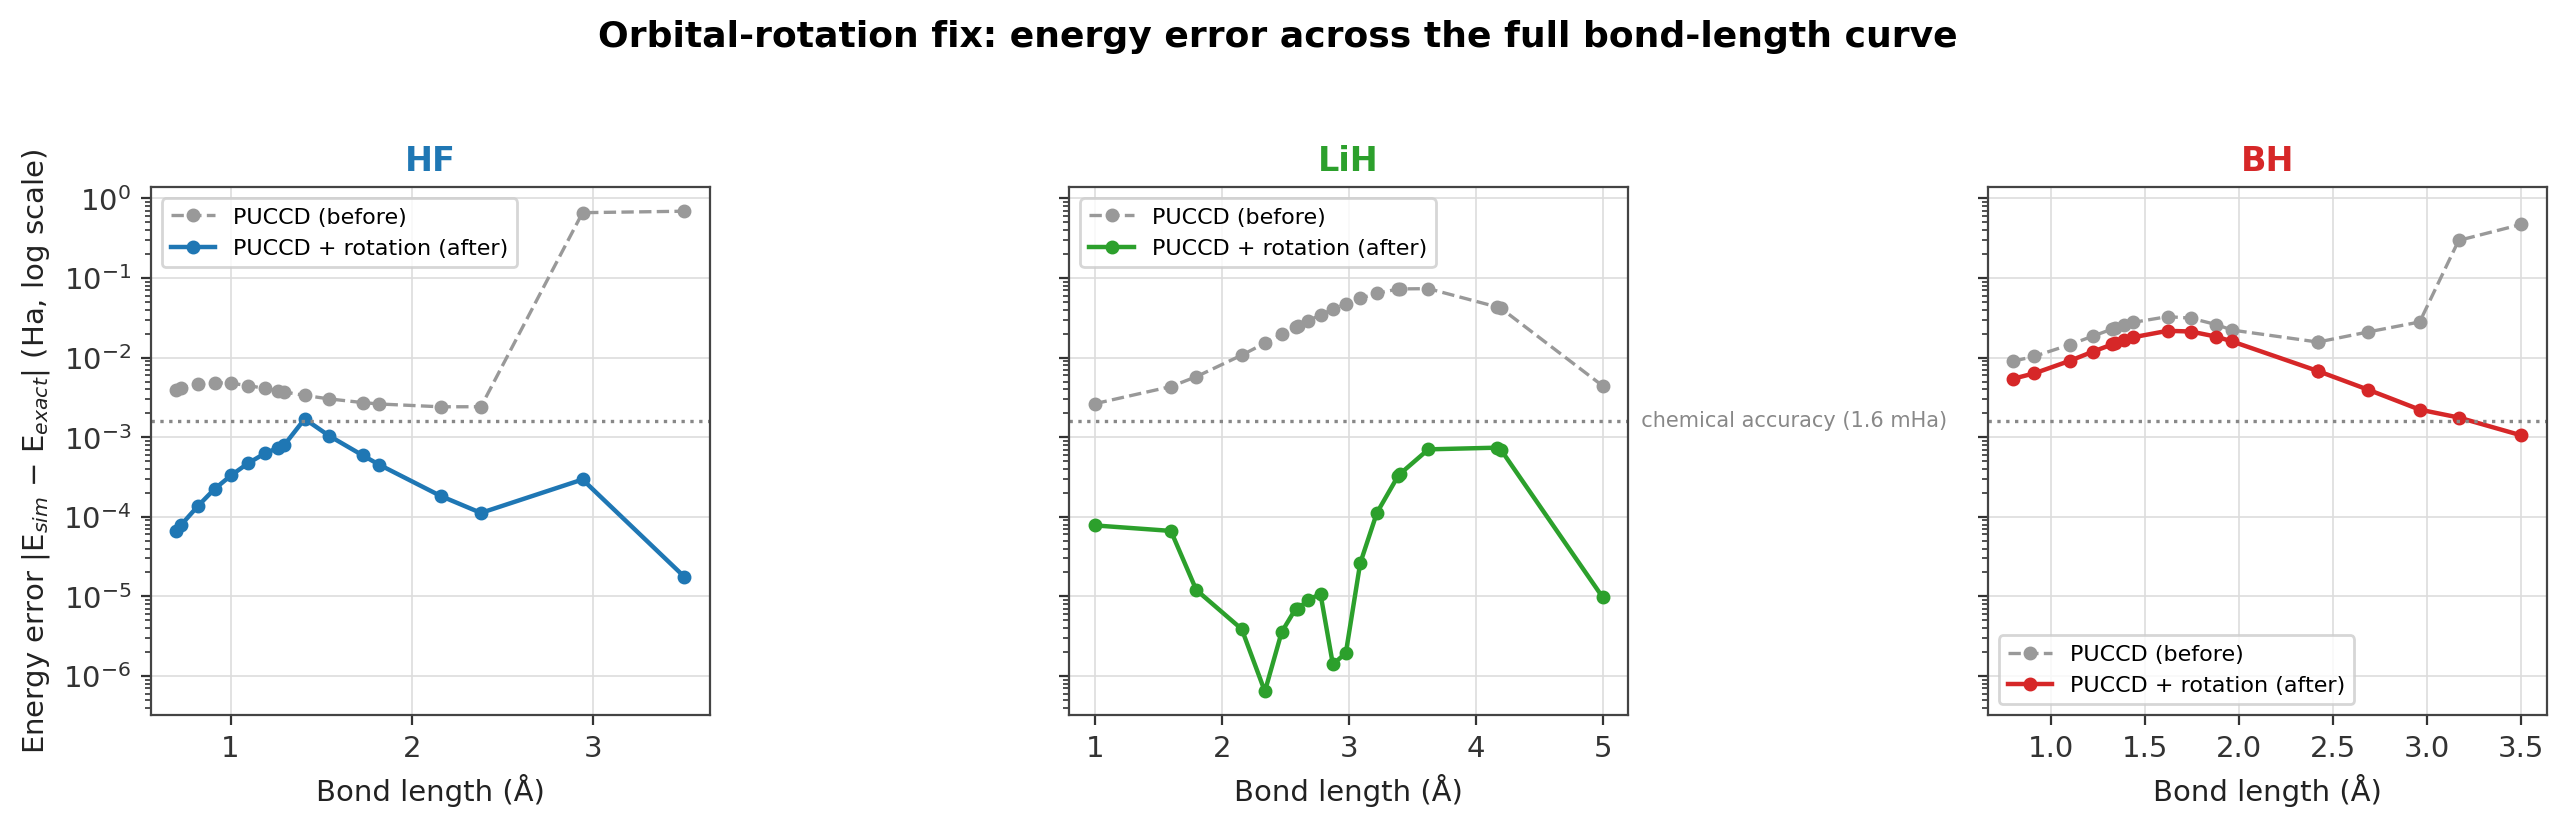
\includegraphics[width=\textwidth]{results_decoupling/figures_proposal/error_reduction_summary.png}
\caption{Energy error (log scale) across the full bond-length curve, before and after the orbital-rotation fix.}
\end{figure}

\begin{table}[h]
\centering
\small
\begin{tabular}{lcccc}
\toprule
Molecule & Geometries tested & Reached chemical accuracy & Max error reduction \\
\midrule
HF  & 17 & 16 / 17 (was 0 / 17) & $\sim$38,766$\times$ \\
LiH & 20 & 20 / 20 (was 0 / 20) & $\sim$28,943$\times$ \\
BH  & 18 & 1 / 18, every point improved & 446$\times$ \\
\bottomrule
\end{tabular}
\caption*{\footnotesize Chemical accuracy threshold: 1.6 mHa. BH's partial result (reported honestly, not rounded up) is itself informative: it suggests boron's valence configuration retains residual multi-reference character that orbital rotation alone does not fully capture, a concrete lead for the proposed extension below.}
\end{table}

\subsection{Ruling out the obvious alternative explanation}
Before attributing the original failures to the ansatz, insufficient optimization was explicitly ruled out: at HF's worst-affected geometries, 12 independent restarts (random and warm-started) converged to the identical energy to within $1\times10^{-6}$ Ha regardless of starting point, a genuine expressibility ceiling, not an under-optimized run. BH and LiH show a rougher multi-restart landscape at a subset of geometries (spreads up to roughly 1 Ha near BH's curve crossing); all reported energies use the best of twelve restarts to control for this.

\section{Proposed extension using Quantum Flywheel resources}
The fix above is validated only in noiseless simulation. The proposed 3-month extension uses exactly the AI-orchestration pattern demonstrated in Section~3, now applied with real QPU access, more compute, and AI-agent-driven search.

\begin{description}[leftmargin=0pt, style=nextline]
\item[Month 1, QPU access.] Validate the fix on real IBM hardware at the 55 decisive geometries (17 HF, 20 LiH, 18 BH), evaluating already-converged simulation parameters once per geometry (no on-hardware re-optimization). The measurement cost is computed, not guessed: each molecule's Jordan-Wigner-mapped 10-qubit Hamiltonian (276 Pauli terms) groups into 58 qubit-wise-commuting circuits, giving a bottom-up budget of $55 \times 58 \times (2{,}000\text{--}4{,}000) \approx$ 6.4 million to 13 million shots. \textit{Success criterion}: hardware energies agree with simulation to within chemical accuracy (1.6 mHa) at a majority of geometries, with any systematic deviation characterized and reported.

\item[Month 2, cloud compute.] Test generalization two ways: three new molecules with qualitatively different bonding (H$_2$O, NH$_3$, CO) in the same tractable qubit range, and one existing molecule re-run in an extended basis (6-31G vs.\ STO-3G). In parallel, target BH's residual gap (Section~4.2) with a small feedforward neural correction (1--2 hidden layers, on the order of 100 parameters) in the style of Li et al., trained on BH's existing 18-geometry dataset. \textit{Success criterion}: the fix's benefit replicates on at least one new molecule or basis, and the correction narrows BH's gap beyond its current $446\times$ best case.

\item[Month 3, AI-agent-orchestrated search.] Rather than hand-selecting excitation operators, use AI-agent-driven search over the untried space, generalized (non-paired) doubles and higher-order singles, targeted at BH's largest-residual geometries. Every candidate is run through the identical audit already validated on the original fix (matched-baseline comparison, twelve-restart consistency check, autocorrelation-corrected statistics from Section~3.2), so a candidate is reported as real only after surviving the same scrutiny the original result did.
\end{description}

\section{Why this is a low-execution-risk proposal}
This is not a cold-start proposal. The pipeline, the statistical methodology, and the diagnostic tooling all already exist and are already validated in simulation; only the hardware-execution step itself (Month 1) is new. The 3-month plan extends a demonstrated, working process rather than building one from scratch. All code, run scripts, raw results, and figures referenced in this document are public: \url{https://github.com/1shaanSr/vqe-ansatz-expressibility}.

\end{document}
